\chapter{Tinjauan Pustaka}
\label{chap:tinjauan-pustaka}

\section{Hasil Penelitian Terdahulu}
\label{sec:hasil-penelitian-terdahulu}

Pada penelitian ini digunakan sejumlah penelitian terdahulu sebagai acuan dalam perancangan dan pengembangan sistem yang diusulkan. Penelitian terdahulu dikelompokkan ke dalam dua kategori utama, yaitu penelitian terkait pengembangan \textit{Smart Attendance System} dan penelitian terkait penerapan \textit{Federated Learning} untuk pengenalan wajah. Ringkasan dari kedua kategori tersebut disajikan pada Tabel \ref{tab:penelitian-smart-attendance} dan Tabel \ref{tab:penelitian-federated-learning}.

\subsection{Penelitian Terkait Pengembangan Smart Attendance System}
\label{subsec:penelitian-smart-attendance}

\begin{longtable}{|c|p{4.5cm}|p{8.5cm}|}
  \caption{Penelitian Terdahulu Terkait Pengembangan Smart Attendance System}\label{tab:penelitian-smart-attendance} \\
  \hline
  \textbf{No} & \textbf{Penulis (Tahun)} & \textbf{Pembahasan} \\
  \hline
  \endfirsthead
  
  \multicolumn{3}{c}{\tablename\ \thetable\ -- \textit{Lanjutan dari halaman sebelumnya}} \\
  \hline
  \textbf{No} & \textbf{Penulis (Tahun)} & \textbf{Pembahasan} \\
  \hline
  \endhead
  
  \hline
  \endfoot
  
  \hline
  \endlastfoot
  
  1 & Srinu et al. (2025) \parencite{Srinu2025} & Penelitian ini mengimplementasikan sistem pencatatan kehadiran cerdas yang mengintegrasikan \textit{Edge Computing} dengan \textit{Convolutional Neural Networks} (CNN) untuk pemrosesan data biometrik secara lokal. Sistem ini menggunakan model FaceNet yang dijalankan pada perangkat \textit{edge} seperti NVIDIA Jetson dan Raspberry Pi untuk meminimalkan latensi serta mengurangi ketergantungan pada layanan \textit{cloud}. Hasil evaluasi menunjukkan kinerja yang sangat baik dengan tingkat akurasi dan presisi mencapai 98,2\%, serta aspek keamanan data yang diperkuat melalui enkripsi AES-256. Peneliti menyarankan penerapan \textit{Federated Learning} di masa mendatang untuk mendesentralisasikan pelatihan model tanpa perlu mentransmisikan data mentah ke \textit{server} pusat. Rekomendasi tersebut menjadi landasan utama bagi penelitian ini untuk melanjutkan pengembangan sistem menggunakan metode \textit{Federated Learning} guna meningkatkan perlindungan privasi data biometrik mahasiswa. \\
  \hline

  2 & Yadav et al. (2021) \parencite{Yadav2021} & Penelitian ini mengimplementasikan arsitektur \textit{Serverless Edge Computing} yang beroperasi sepenuhnya pada lingkungan \textit{in-browser} guna memitigasi isu latensi dan privasi dalam pembelajaran daring. Sistem dirancang sebagai solusi presensi yang ringan dan \textit{cost-effective} tanpa ketergantungan pada perangkat keras khusus, dengan memanfaatkan pustaka face-api.js dan TensorFlow.js. Pendekatan ini memungkinkan eksekusi model \textit{deep learning}, seperti Tiny Face Detector dan Face Recognition Net, dilakukan langsung di sisi \textit{client} dengan integrasi Google Sheets untuk manajemen basis data. Hasil evaluasi menunjukkan sistem memiliki performa responsif dengan waktu pemrosesan antara 2 hingga 3 detik dan mampu memvalidasi kehadiran menggunakan \textit{confidence threshold} di atas 65\%. \\
  \hline
\end{longtable}

\subsection{Penelitian Terkait Federated Learning untuk Pengenalan Wajah}
\label{subsec:penelitian-federated-learning}

\begin{longtable}{|c|p{4.5cm}|p{8.5cm}|}
  \caption{Penelitian Terdahulu Terkait Federated Learning untuk Pengenalan Wajah}\label{tab:penelitian-federated-learning} \\
  \hline
  \textbf{No} & \textbf{Penulis (Tahun)} & \textbf{Pembahasan} \\
  \hline
  \endfirsthead
  
  \multicolumn{3}{c}{\tablename\ \thetable\ -- \textit{Lanjutan dari halaman sebelumnya}} \\
  \hline
  \textbf{No} & \textbf{Penulis (Tahun)} & \textbf{Pembahasan} \\
  \hline
  \endhead
  
  \hline
  \endfoot
  
  \hline
  \endlastfoot
  
  1 & Gao et al. (2025) \parencite{Gao2025} & Penelitian ini memperkenalkan kerangka kerja pFedFace yang dirancang untuk menyeimbangkan antara generalisasi model global dengan kebutuhan personalisasi lokal pada sistem pengenalan wajah. Inovasi utama yang diusulkan adalah skema \textit{Adaptive Batch Normalization} (BN) yang memisahkan setiap lapisan BN menjadi dua varian: varian generik untuk mencapai konsensus global dan varian spesifik \textit{client} untuk adaptasi domain lokal. Hasil evaluasi pada \textit{benchmark} skala besar menunjukkan bahwa pFedFace berhasil meningkatkan akurasi antara 1,0\% hingga 2,68\% dibandingkan metode \textit{baseline} seperti FedAvg, serta mencapai akurasi 93,35\% pada subset tertentu. Strategi ini diimplementasikan dalam penelitian ini melalui mekanisme pemisahan parameter \textit{batch normalization} pada arsitektur MobileFaceNet. Dengan pendekatan tersebut, proses agregasi hanya dilakukan pada parameter \textit{backbone} model, sementara lapisan BN dikelola secara lokal pada perangkat Raspberry Pi dan Jetson Nano untuk mengoptimalkan akurasi pengenalan identitas mahasiswa secara personal di setiap titik kehadiran. \\
  \hline

  2 & Gupta \& Singh (2025) \parencite{Gupta2025} & Penelitian ini mengusulkan sebuah kerangka kerja sistem pengenalan wajah berorientasi \textit{Internet of Things} (IoT) yang menggabungkan arsitektur hibrida \textit{Convolutional Neural Network} (CNN)-Transformer dengan metode \textit{Federated Edge Learning}. Metodologi ini memanfaatkan MobileNetV3 sebagai \textit{backbone} CNN untuk ekstraksi fitur spasial lokal yang kemudian diintegrasikan dengan \textit{transformer encoder} ringan untuk pemodelan konteks wajah secara global. Proses pelatihan dilakukan secara terdesentralisasi antar \textit{node} IoT menggunakan fungsi \textit{ArcFace margin loss} dan algoritma agregasi dengan teknik \textit{gradient sparsification} untuk meminimalkan beban \textit{bandwidth} komunikasi. Hasil evaluasi komprehensif pada dataset LFW menunjukkan tingkat akurasi yang tinggi mencapai 98,2\%, serta mampu mempertahankan akurasi sebesar 96,7\% di bawah kondisi wajah yang terhalang (\textit{occlusion}). Selain itu, ketika diimplementasikan pada perangkat \textit{edge} seperti Raspberry Pi 4 melalui \textit{Quantization-Aware Training} (QAT) INT8, sistem ini berhasil memangkas latensi inferensi hingga menjadi 45 milidetik dan mengurangi konsumsi energi menjadi 290 mJ per inferensi. \\
  \hline
\end{longtable}

\section{Dasar Teori}
\label{sec:dasar-teori}

\subsection{Federated Learning}
\label{subsec:federated-learning-teori}

\textit{Federated Learning} merupakan pendekatan \textit{machine learning} terdesentralisasi yang memungkinkan beberapa perangkat berkolaborasi untuk melatih satu model bersama tanpa mengirimkan data mentah ke \textit{server} pusat. Setiap \textit{client} melakukan pelatihan model secara lokal dan hanya mengirimkan pembaruan model, seperti parameter atau gradien untuk diagregasi secara terpusat. Pendekatan ini menjaga privasi data sekaligus mengurangi ketergantungan pada penyimpanan terpusat \parencite{Shaheen2022}.

Arsitektur umum \textit{Federated Learning} dapat dilihat pada Gambar \ref{fig:federated-learning}. Prosesnya berjalan secara berulang sampai model mencapai konvergensi. Secara umum, terdapat empat tahapan utama, yaitu:
\begin{enumerate}[itemsep=1pt]
  \item \textit{Server} mengirimkan model global ke seluruh \textit{client}.
  \item \textit{Client} melakukan pelatihan model menggunakan data lokal.
  \item \textit{Client} mengirimkan pembaruan model ke \textit{server}.
  \item \textit{Server} melakukan agregasi untuk menghasilkan model global yang diperbarui.
\end{enumerate}

\begin{figure}[H]
  \centering
  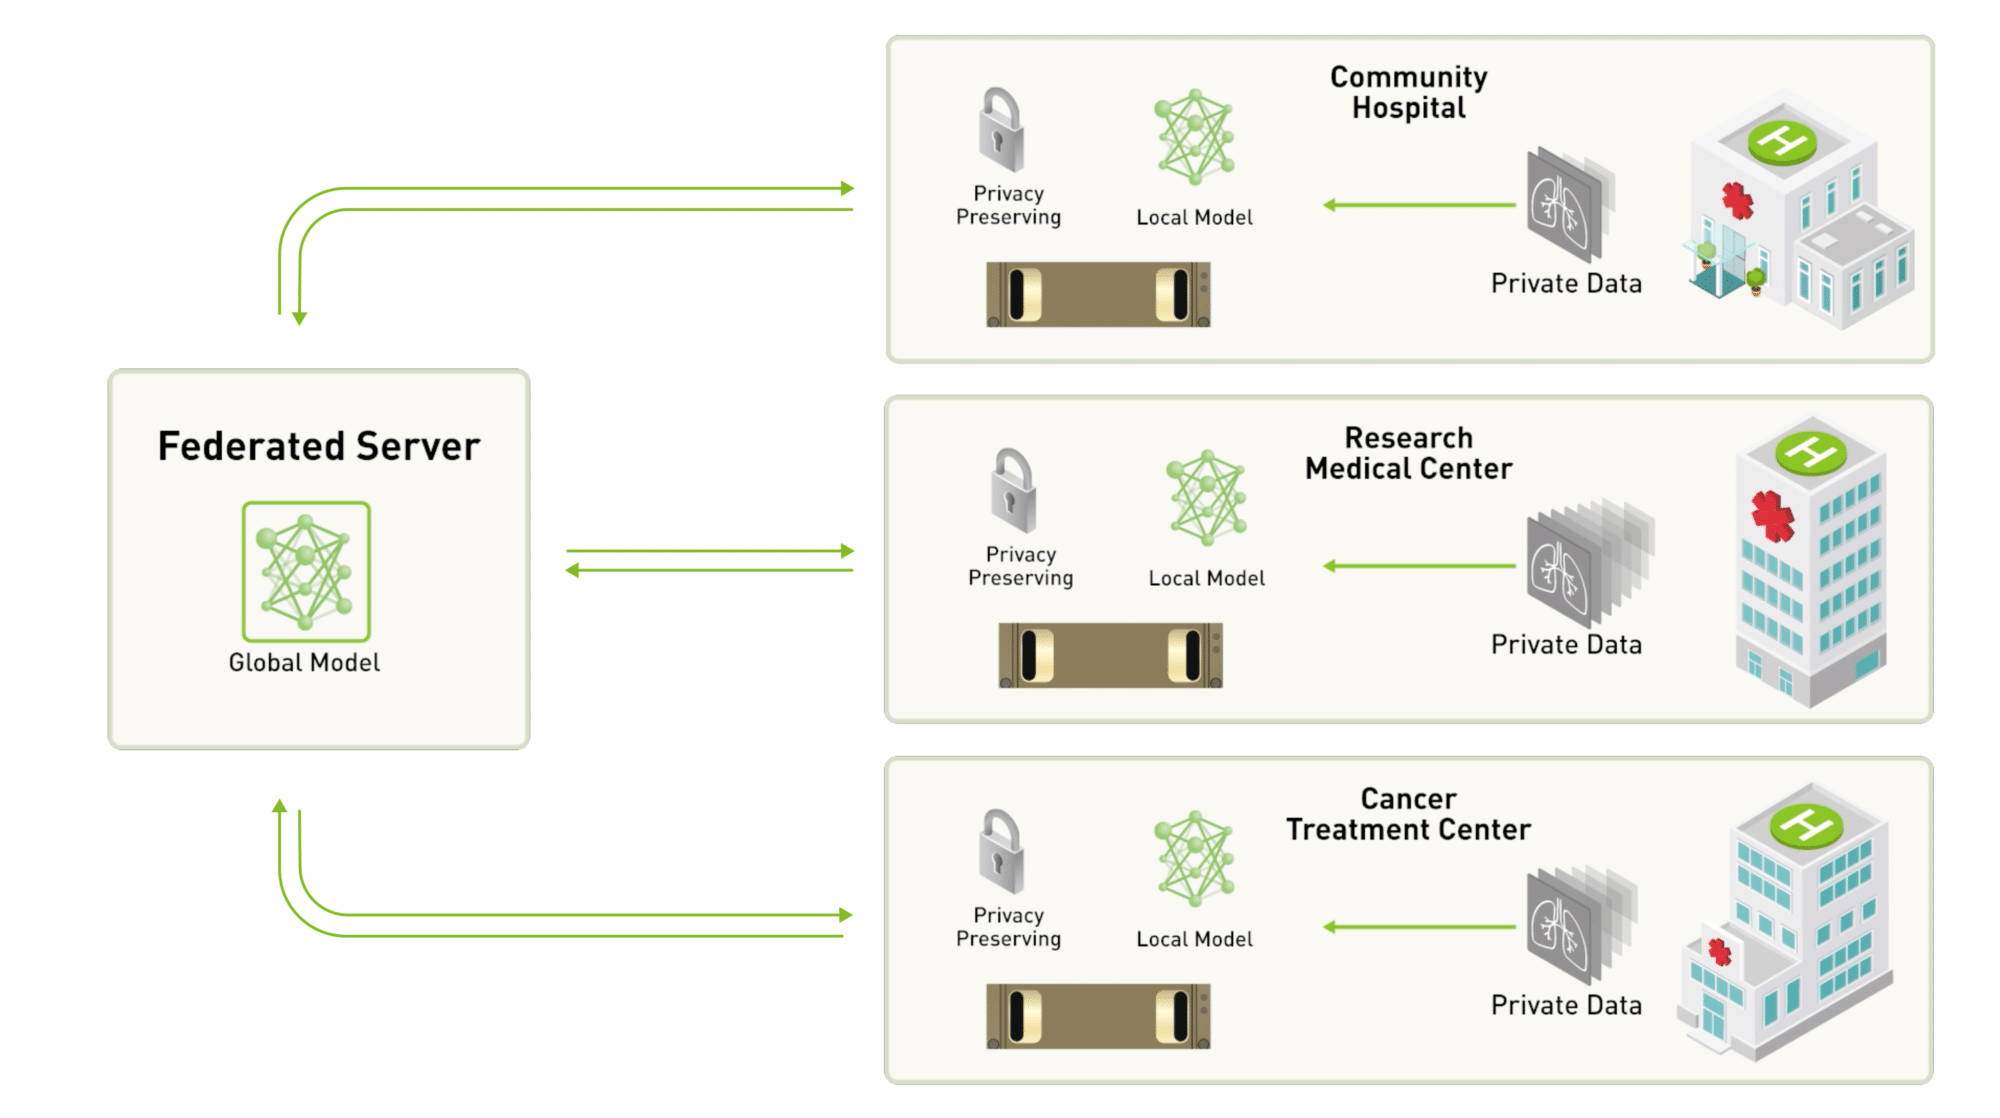
\includegraphics[width=0.7\textwidth]{gambar/Federated_Learning.png}
  \caption{Arsitektur Umum \textit{Federated Learning}}
  \label{fig:federated-learning}
\end{figure}
\begin{center}
  Sumber: \parencite{NVIDIA2019}
\end{center}

Dibandingkan dengan \textit{Centralized Learning}, \textit{Federated Learning} menawarkan beberapa keunggulan utama, yaitu:
\begin{enumerate}[itemsep=1pt]
  \item Peningkatan privasi karena data tetap berada pada perangkat \textit{edge} masing-masing.
  \item Pengurangan beban komunikasi jaringan karena yang dikirim adalah pembaruan model.
  \item Mitigasi masalah \textit{data silos}, yaitu kondisi ketika data tersebar pada berbagai perangkat sehingga tidak dapat digabungkan secara langsung untuk pelatihan terpusat.
\end{enumerate}

\textit{Federated Learning} merupakan konsep utama yang diterapkan dalam penelitian ini untuk memungkinkan proses pelatihan model pengenalan wajah dilakukan secara terdistribusi pada perangkat \textit{edge}. Melalui pendekatan ini, privasi data biometrik tetap terjaga di tingkat lokal, sekaligus mengatasi tantangan heterogenitas data (non-IID) yang umum terjadi pada sistem kehadiran di lingkungan \textit{edge computing}.

Perlu dicatat bahwa implementasi \textit{Federated Learning} dalam penelitian ini berbeda dengan skenario ideal pada literatur, di mana data diasumsikan telah tersedia secara asli di masing-masing perangkat \textit{client}. Pada penelitian ini, pengumpulan data awal dilakukan secara terpusat menggunakan \textit{laptop} di mana video wajah mahasiswa direkam menggunakan \textit{webcam} dan diekstraksi menjadi kumpulan \textit{frame} yang kemudian didistribusikan secara manual ke setiap perangkat \textit{edge} sebelum pelatihan dimulai. Siklus \textit{Federated Learning} yang sesungguhnya baru berjalan mulai dari tahap \textit{preprocessing} di masing-masing perangkat \textit{client}, kemudian dilanjutkan dengan pelatihan model lokal, agregasi parameter di \textit{server}, dan inferensi kehadiran secara \textit{real-time}. Dengan demikian, citra wajah asli tidak pernah meninggalkan perangkat \textit{edge} selama siklus \textit{Federated Learning} berlangsung.

\subsection{Centralized Learning}
\label{subsec:centralized-learning-teori}

\textit{Centralized Learning} merupakan pendekatan pembelajaran mesin konvensional di mana seluruh data yang dikumpulkan dari berbagai sumber harus ditransmisikan dan disimpan dalam satu \textit{server} pusat untuk menjalani proses pelatihan model. Dalam arsitektur ini, unit pemrosesan terpusat memiliki kendali penuh atas dataset, yang memungkinkannya untuk melakukan pengoptimalan model secara global dengan visibilitas data yang menyeluruh \parencite{Tertulino2025}.

Dalam penelitian ini, \textit{Centralized Learning} diterapkan sebagai standar pembanding (\textit{baseline}) untuk mengevaluasi performa model MobileFaceNet, guna mengukur sejauh mana efektivitas dan akurasi yang dihasilkan oleh \textit{Federated Learning} dibandingkan dengan metode pelatihan terpusat tersebut.

\subsection{Flower}
\label{subsec:flower-teori}

Flower adalah salah satu kerangka kerja \textit{Federated Learning} yang dirancang untuk menghubungkan tahap simulasi riset dengan penerapan sistem di perangkat \textit{edge}. Keunggulan utamanya adalah sifatnya yang agnostik, artinya kerangka kerja ini tidak terikat atau bergantung pada satu pustaka \textit{machine learning} tertentu. Pengguna bebas menggunakan tools seperti TensorFlow, PyTorch, atau lainnya tanpa masalah kompatibilitas. Fleksibilitas ini sangat memudahkan proses pemindahan kode dari tahap eksperimen ke implementasi dunia nyata tanpa perlu melakukan perombakan besar pada struktur dasarnya \parencite{Beutel2022}.

\begin{figure}[H]
  \centering
  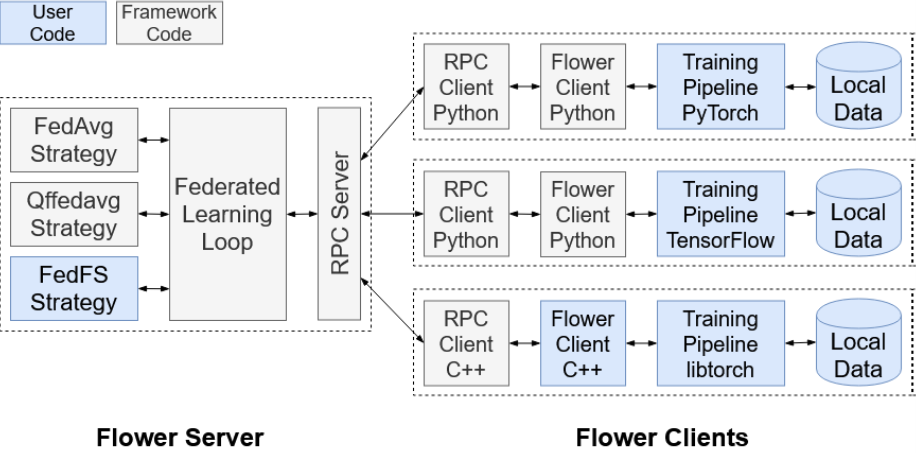
\includegraphics[width=0.7\textwidth]{gambar/Flower.png}
  \caption{Arsitektur Flower}
  \label{fig:arsitektur-flower}
\end{figure}
\begin{center}
  Sumber: \parencite{Mathur2021}
\end{center}

Arsitektur Flower seperti ditunjukkan pada Gambar \ref{fig:arsitektur-flower}, memisahkan fungsi \textit{server} sebagai pengatur pusat dan \textit{client} sebagai pelaksana pelatihan di perangkat. Komunikasi antar komponen menggunakan protokol gRPC, yang mendukung pertukaran data pada perangkat dengan sumber daya terbatas. Dalam penelitian ini, Flower digunakan untuk menangani komunikasi data.

\subsection{FedProx}
\label{subsec:fedprox-teori}

Algoritma \textit{Federated Proximal} (FedProx) hadir sebagai bentuk pengembangan dari metode konvensional \textit{Federated Averaging} (FedAvg) untuk mengatasi kendala heterogenitas pada jaringan terdistribusi. Konsep utama dari FedProx adalah restrukturisasi pada fungsi objektif lokal di setiap perangkat \textit{client} dengan menambahkan sebuah komponen penalti matematis yang disebut \textit{proximal term} ($\mu$). Mekanisme ini dirancang untuk membatasi arah pembaruan parameter selama pelatihan lokal agar tidak melenceng terlalu jauh dari arsitektur model global yang dikelola oleh \textit{server} pusat. Melalui pendekatan ini, stabilitas dan konsistensi konvergensi model dapat tetap terjaga dengan baik meskipun data yang tersebar di lapangan bersifat tidak seragam (Non-IID). Fungsi objektif lokal utama FedProx dirumuskan melalui Persamaan (\ref{eq:fedprox-obj}) berikut:
\begin{equation}
  \label{eq:fedprox-obj}
  \min_{w_k} \left[ F_k(w_k) + \frac{\mu}{2} \|w_k - w^g\|^2 \right]
\end{equation}

Keterangan:
\begin{itemize}[itemsep=1pt]
  \item $w_k$: representasi matriks parameter model lokal pada \textit{client} ke-$k$.
  \item $w^g$: bobot model global saat itu.
  \item $F_k(w_k)$: nilai fungsi loss lokal yang dihitung berdasarkan data privat masing-masing perangkat.
  \item $\mu$: Koefisien regularisasi \textit{proximal parameter} yang mengontrol batas deviasi bobot model.
  \item $\|w_k - w^g\|^2$: menyatakan kuadrat jarak $L_2$ antara bobot lokal dan global.
\end{itemize}

Proses komputasi pada skema FedProx berjalan melalui tiga tahapan siklus iteratif yang ketat. Tahap pertama dimulai dari \textit{Server-Side Broadcast}, di mana \textit{server} membagikan parameter model global mutakhir ($w^g$) kepada seluruh perangkat klien yang terpilih. Masuk ke tahap kedua, yaitu \textit{Local Optimization}, setiap \textit{client} menghitung nilai error dari fungsi loss lokal berbasis data privatnya ($F_k(w)$) menggunakan metode rata-rata sampel melalui Persamaan (\ref{eq:fedprox-loss}) berikut:
\begin{equation}
  \label{eq:fedprox-loss}
  F_k(w_k) = \frac{1}{n_k} \sum_{x_i, y_i \in D_k} l(w_k; x_i, y_i)
\end{equation}

Keterangan:
\begin{itemize}[itemsep=1pt]
  \item $n_k$: Jumlah total sampel data latih yang dimiliki dan diisolasi oleh \textit{client} ke-$k$.
  \item $D_k$: Kumpulan dataset lokal pada penyimpanan perangkat \textit{client} ke-$k$.
  \item $l(w_k; x_i, y_i)$: Fungsi loss dasar yang dihitung untuk setiap satu sampel data tunggal.
\end{itemize}

Berbeda dengan FedAvg konvensional yang membiarkan \textit{client} melakukan optimasi loss lokal secara bebas, komponen \textit{proximal term} pada fungsi objektif utama FedProx bertindak sebagai pengekang matematis. Komponen ini memberikan nilai penalti yang semakin besar apabila arah pergeseran bobot lokal ($w_k$) menjauh dari jangkar model global ($w^g$).

Setelah iterasi pelatihan lokal selesai, proses memasuki tahap ketiga berupa \textit{Weighted Aggregation}. Seluruh koordinasi parameter bobot yang dikirimkan oleh perangkat \textit{edge} akan dikumpulkan dan diakumulasikan kembali oleh \textit{server} pusat untuk memperbarui parameter model global pada ronde berikutnya ($w^{t+1}_{global}$) melalui mekanisme rata-rata tertimbang (\textit{weighted averaging}) menggunakan Persamaan (\ref{eq:fedprox-agg}) berikut:
\begin{equation}
  \label{eq:fedprox-agg}
  w^{t+1}_{global} = \sum_{k=1}^{K} \frac{n_k}{N} w_k^{(t)}
\end{equation}

Keterangan:
\begin{itemize}[itemsep=1pt]
  \item $K$: Jumlah total seluruh perangkat \textit{client} yang berpartisipasi aktif dalam pelatihan.
  \item $N$: Akumulasi total volume data dari gabungan seluruh \textit{client} yang terdaftar.
  \item $w_k^{(t)}$: Matriks parameter bobot lokal hasil latih dari \textit{client} ke-$k$ setelah menyelesaikan ronde ke-$t$.
\end{itemize}

Penentuan nilai besaran parameter hiperparameter $\mu$ (regularisasi \textit{proximal term}) memiliki pengaruh yang sangat sensitif dan berbanding terbalik terhadap stabilitas serta karakteristik konvergensi model di lapangan. Jika nilai $\mu$ diatur terlalu besar, tali pengekang model akan menjadi sangat kaku; sistem dipaksa untuk terus menyerupai model global sehingga proses pembaruan bobot lokal menjadi lambat, menghambat model untuk mempelajari variasi fitur wajah baru, dan berisiko memperlama durasi pencapaian konvergensi sistem. Sebaliknya, apabila nilai $\mu$ diturunkan hingga mendekati angka nol, sifat bawaan FedProx akan luruh dan sistem kembali beroperasi layaknya algoritma FedAvg biasa. Dalam kondisi data lokal yang tidak seragam (Non-IID), nilai $\mu$ yang terlalu kecil akan membuat setiap perangkat \textit{edge} memperbarui parameter secara agresif demi meminimalkan loss lokalnya sendiri, yang berujung pada fenomena \textit{client drift} (pergeseran bobot lokal yang saling bertolak belakang), perlambatan akurasi global, hingga risiko kegagalan latih (\textit{divergence}). Oleh karena itu, nilai $\mu$ harus dikunci pada angka yang optimal guna menyeimbangkan fleksibilitas adaptasi lokal di setiap node edge tanpa mengorbankan stabilitas akurasi model global \parencite{Xiong2025}.

Dalam penelitian sistem kehadiran mahasiswa ini, FedProx diterapkan sebagai algoritma agregasi utama untuk mengorkestrasi pembaruan parameter model dari berbagai perangkat keras \textit{edge} secara aman dan konsisten.

\subsection{pFedFace}
\label{subsec:pfedface-teori}

pFedFace adalah kerangka kerja \textit{personalized federated learning} yang dirancang khusus untuk mengatasi keterbatasan metode FL konvensional dalam pengenalan wajah, di mana metode konvensional hanya berfokus pada pembentukan representasi wajah secara global tanpa mempertimbangkan kebutuhan personalisasi lokal masing-masing \textit{client} \parencite{Gao2025}. Inovasi utamanya adalah skema \textit{Adaptive Batch Normalization} (BN) yang menduplikasi setiap lapisan BN menjadi dua varian. Varian pertama bersifat generik dan berperan menyatukan pengetahuan antar-\textit{client} untuk generalisasi global, sedangkan varian kedua bersifat spesifik per-\textit{client} dan bertugas menjembatani perbedaan domain antar-perangkat untuk personalisasi lokal. Selain itu, pFedFace memperkenalkan \textit{personalized discriminative loss} yang mendorong model lokal untuk mengekstraksi fitur wajah secara lebih diskriminatif dibandingkan model global.

Dalam penelitian ini, strategi pFedFace diterapkan melalui mekanisme pemisahan parameter \textit{Batch Normalization} pada arsitektur MobileFaceNet. Secara praktis, pada saat proses agregasi berlangsung, hanya bobot lapisan konvolusi (\textit{backbone}) yang dikirim ke \textit{server} dan diagregasi menjadi model global. Lapisan BN beserta statistiknya (\textit{running mean} dan \textit{running variance}) tidak ikut dikirim dan tetap dikelola secara lokal di masing-masing perangkat \textit{edge}, yaitu Raspberry Pi dan Jetson Nano. Dengan cara ini, setiap perangkat dapat mempertahankan kalibrasi statistik normalisasinya terhadap kondisi kamera dan pencahayaan lokalnya masing-masing, sehingga akurasi inferensi identitas mahasiswa di setiap titik kehadiran dapat dioptimalkan secara personal tanpa mengorbankan pengetahuan global yang diperoleh melalui agregasi.

\subsection{Face Recognition}
\label{subsec:face-recognition-teori}

\textit{Face Recognition} atau pengenalan wajah adalah teknik biometrik yang digunakan untuk mengidentifikasi atau memverifikasi seseorang berdasarkan fitur wajah yang diproses melalui model \textit{deep learning}. Kemajuan \textit{deep learning} membuat akurasinya meningkat, tetapi pelatihan model biasanya membutuhkan banyak data wajah yang bersifat sensitif dan sulit dibagikan. Hal ini menjadikan pengenalan wajah sebagai bidang yang membutuhkan pendekatan pembelajaran yang aman dan terdistribusi \parencite{Kim2021}.

Dalam penelitian ini, pengenalan wajah digunakan sebagai inti sistem absensi. Proses identifikasi dijalankan langsung pada perangkat \textit{edge}. Dengan cara ini, sistem dapat bekerja lebih cepat dan tetap menjaga kerahasiaan data biometrik.

\subsection{MobileFaceNet}
\label{subsec:mobilefacenet-teori}

MobileFaceNet merupakan arsitektur \textit{deep learning} yang dirancang untuk pengenalan wajah pada perangkat dengan sumber daya terbatas. Model ini termasuk jaringan ringan (\textit{lightweight CNN}) yang fokus pada efisiensi komputasi tanpa mengorbankan akurasi secara signifikan. MobileFaceNet menggunakan teknik seperti \textit{depthwise separable convolution} yang membuat ukuran model kecil namun tetap mampu mengekstraksi fitur wajah dengan baik \parencite{Xiao2024}.

Dalam penelitian ini, MobileFaceNet diimplementasikan sebagai model utama untuk pengenalan wajah pada sistem kehadiran. Penelitian ini menerapkan strategi \textit{transfer learning} dengan memanfaatkan bobot awal (\textit{pre-trained weights}) yang bersumber dari implementasi \textit{open-source} MobileFaceNet berbasis PyTorch oleh \textcite{Xiaoccer2023} yang dilatih menggunakan dataset CASIA-WebFace dan dievaluasi menggunakan dataset LFW (\textit{Labelled Faces in the Wild}). Penggunaan bobot awal ini berfungsi sebagai inisialisasi dasar untuk mempercepat konvergensi sebelum dilakukan proses \textit{Federated Learning}. Model ini dipilih karena karakteristiknya yang ringan, sehingga mampu beroperasi secara optimal dan efisien pada perangkat \textit{edge} yang memiliki keterbatasan sumber daya komputasi.

\subsection{Face Embedding}
\label{subsec:face-embedding-teori}

\textit{Face Embedding} adalah proses ekstraksi fitur biometrik di mana citra wajah mentah ditransformasikan oleh jaringan saraf tiruan mendalam menjadi sebuah vektor numerik berdimensi tinggi yang unik. Vektor ini merepresentasikan karakteristik geometris wajah individu secara abstrak, sehingga proses pengenalan identitas tidak lagi membandingkan gambar piksel demi piksel, melainkan cukup dengan menghitung kedekatan jarak matematis antar vektor embedding tersebut, meskipun representasi data ini lebih ringkas dibandingkan citra asli \parencite{Shahreza2025}.

Dalam penelitian ini, \textit{face embedding} yang dihasilkan oleh arsitektur MobileFaceNet digunakan sebagai representasi data utama untuk melakukan verifikasi pada sistem kehadiran mahasiswa.

\subsection{MTCNN}
\label{subsec:mtcnn-teori}

MTCNN atau \textit{Multi-task Convolutional Neural Network} adalah model jaringan saraf \textit{multi-task} yang dirancang untuk melakukan deteksi wajah dengan menyeimbangkan kinerja dan akurasi. Algoritma ini menggunakan struktur jaringan berjenjang yang terdiri dari tiga lapisan, yaitu P-Net (\textit{Proposal Network}), R-Net (\textit{Refine Network}), dan O-Net (\textit{Output Network}). Mekanisme kerjanya dimulai dengan menghasilkan kandidat kotak area target menggunakan model kecil, yang kemudian disaring secara bertahap menggunakan model yang lebih kompleks untuk mendapatkan klasifikasi dan regresi kotak pembatas wajah yang presisi \parencite{Zhang2020}.

Dalam penelitian ini, MTCNN digunakan sebagai metode utama pada tahap \textit{preprocessing} untuk mendeteksi dan \textit{cropping} area wajah dari citra asli. Kemampuan MTCNN dalam menyaring kandidat area wajah (\textit{bounding box}) digunakan untuk memastikan bahwa input yang akan dimasukkan ke dalam model MobileFaceNet hanyalah bagian wajah yang bersih dan akurat.

\subsection{Edge Computing}
\label{subsec:edge-computing-teori}

\textit{Edge Computing} adalah arsitektur komputasi terdistribusi di mana pemrosesan data dilakukan secara lokal, dekat dengan sumber datanya. Karena tidak semua data dikirim ke \textit{cloud}, pendekatan ini bisa mengurangi latensi, menghemat \textit{bandwidth}, dan memungkinkan aplikasi yang butuh respon cepat berjalan lebih efisien \parencite{Brecko2022}.

Penelitian ini memanfaatkan \textit{edge computing} sebagai dasar perancangan sistem. Pemrosesan dilakukan langsung pada perangkat \textit{edge}, sehingga identifikasi wajah bisa berlangsung secara lokal.

\begin{figure}[H]
  \centering
  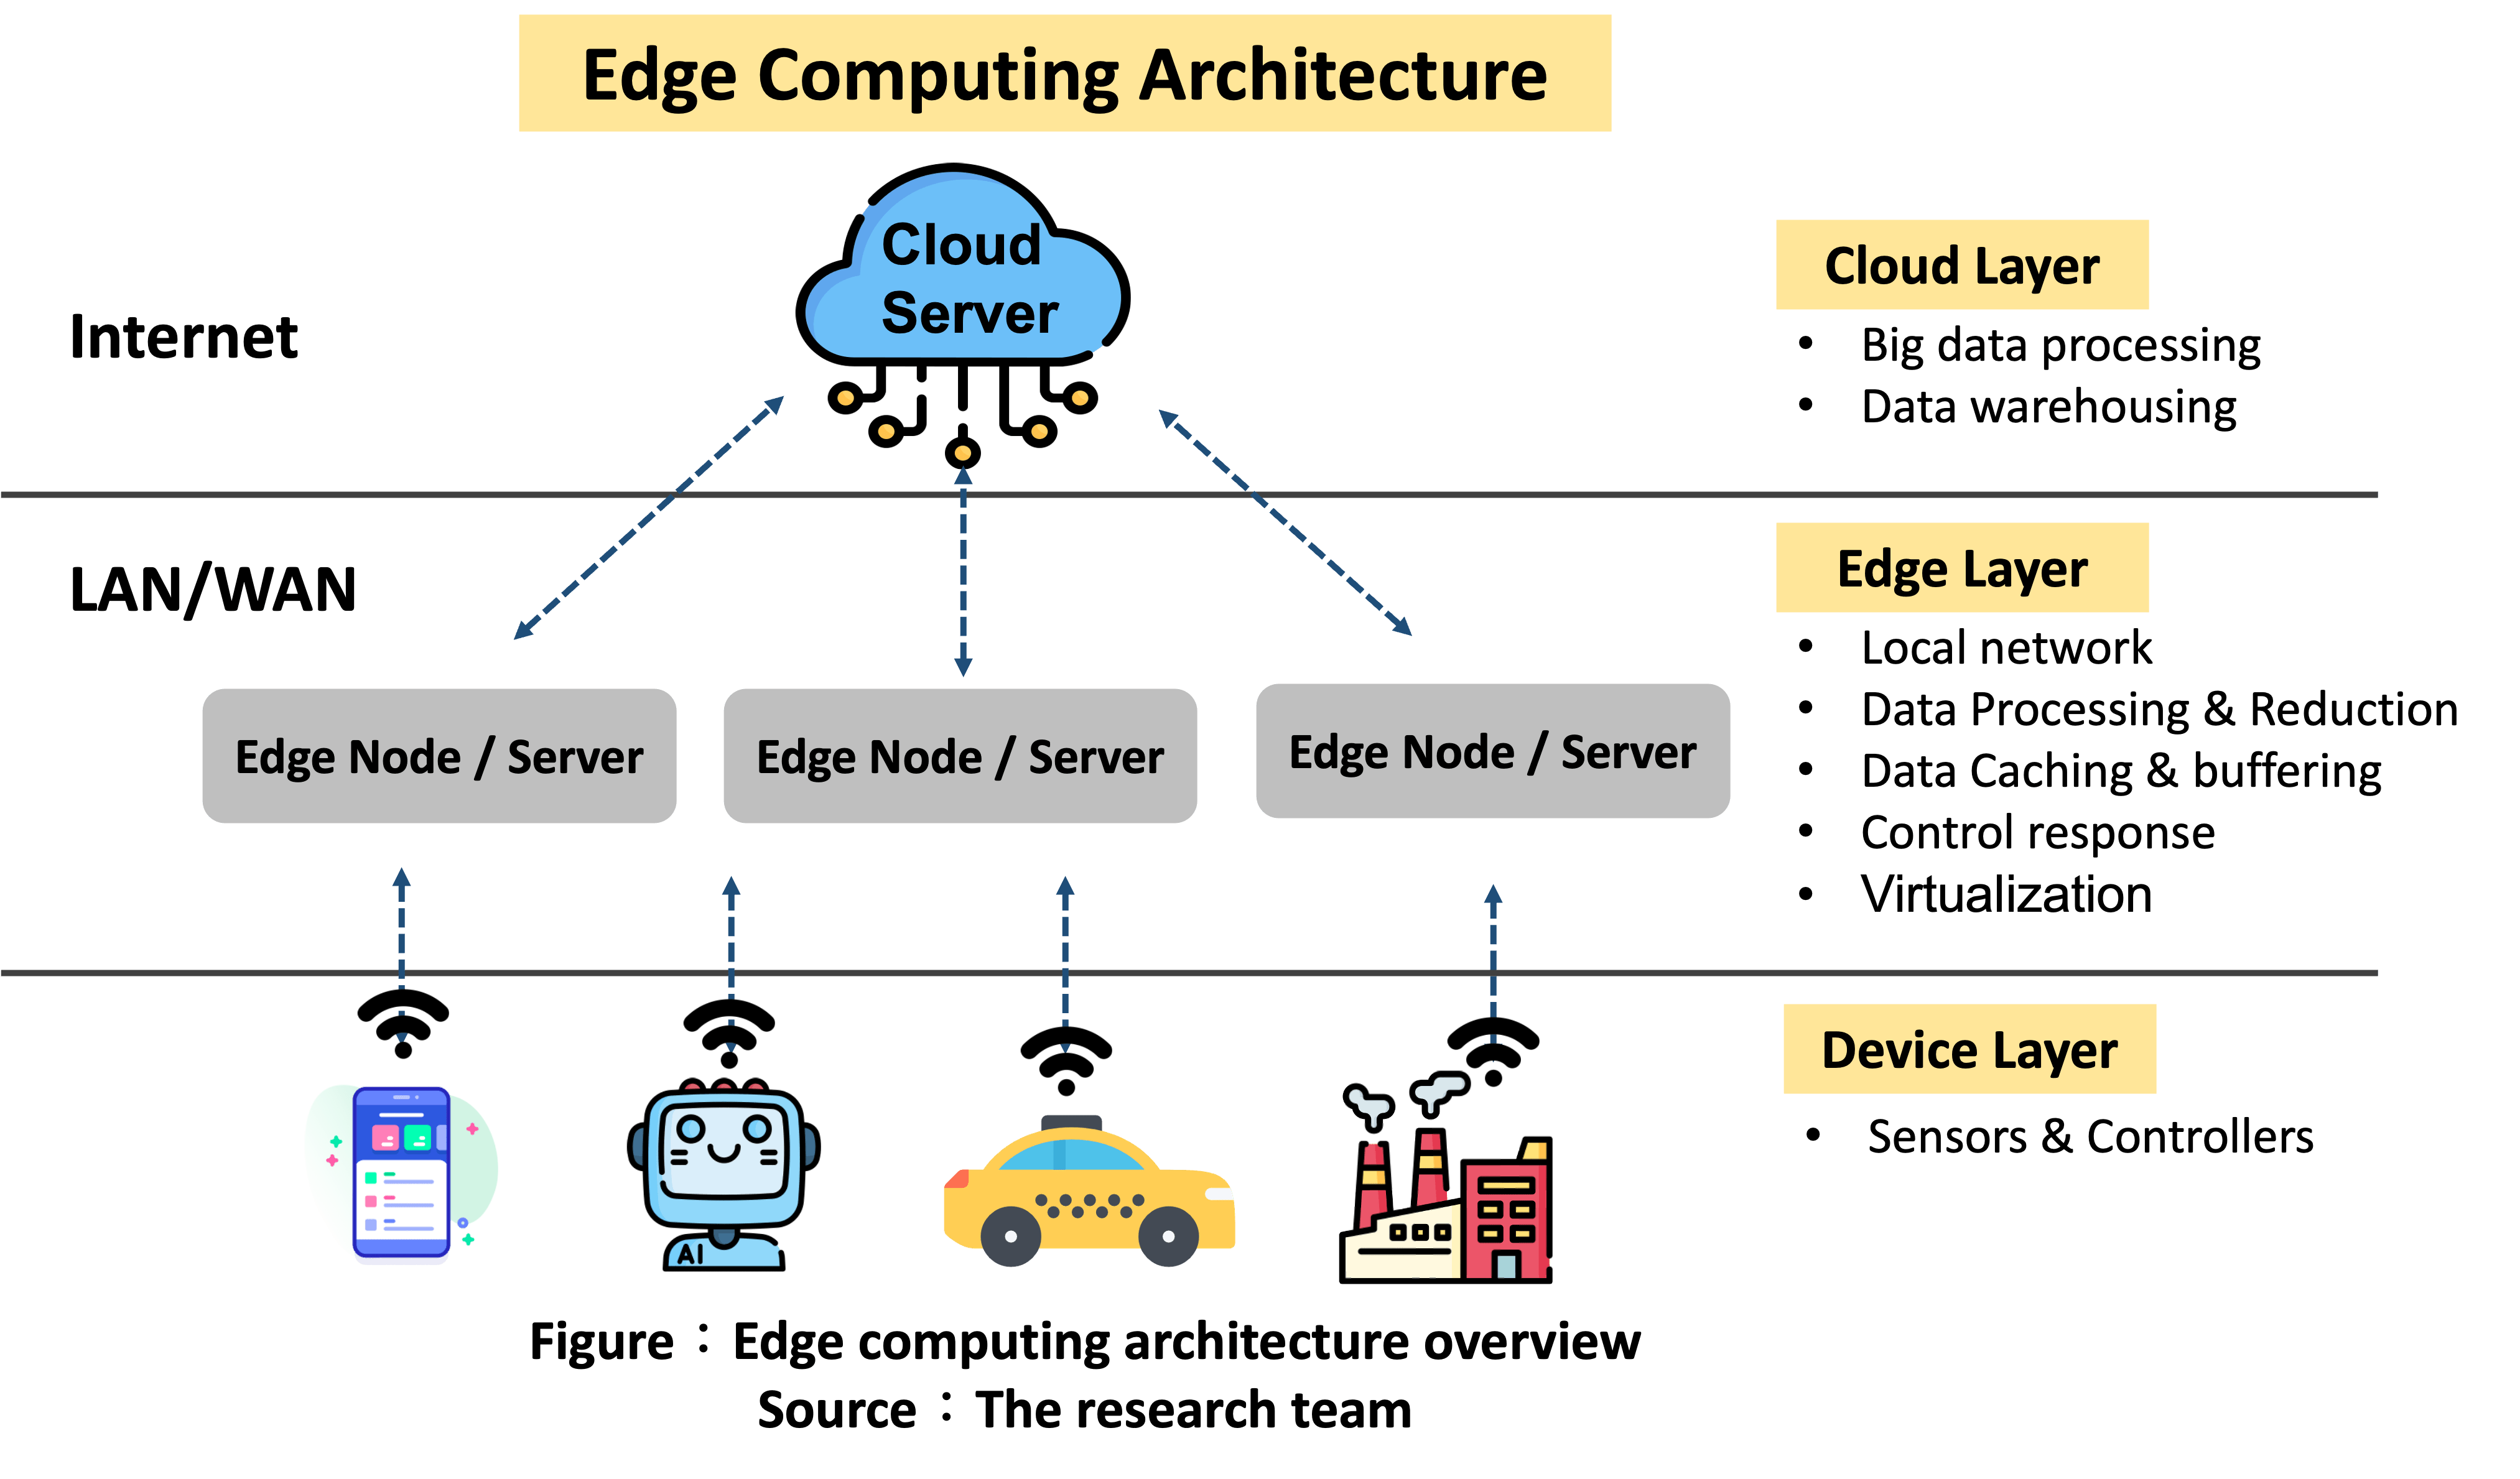
\includegraphics[width=0.7\textwidth]{gambar/Edge_Computing.png}
  \caption{Arsitektur Edge Computing}
  \label{fig:edge-computing}
\end{figure}
\begin{center}
  Sumber: \parencite{FSPGroup2021}
\end{center}

\subsection{Docker}
\label{subsec:docker-teori}

Docker adalah sebuah platform \textit{containerization} yang memungkinkan aplikasi dijalankan dalam lingkungan terisolasi yang disebut container. Setiap container membawa aplikasi beserta dependensinya, sehingga aplikasi dapat berjalan konsisten di berbagai perangkat tanpa konflik konfigurasi \parencite{Nandi2023}.

Dalam penelitian ini, Docker digunakan untuk menjalankan dan mengelola komponen aplikasi dalam lingkungan yang seragam. Penggunaan container membantu mengurangi perbedaan konfigurasi antarperangkat dan mempermudah proses pengembangan serta implementasi.

\subsection{AES-256}
\label{subsec:aes256-teori}

AES-256 adalah varian dari standar enkripsi simetris \textit{Advanced Encryption Standard} (AES) yang ditetapkan oleh NIST, yang beroperasi menggunakan panjang kunci 256-bit. Algoritma ini memproses data dalam blok 128-bit melalui 14 \textit{rounds} enkripsi, jumlah yang lebih banyak dibandingkan varian standar 128-bit \parencite{Gonzalez2023}.

Dalam penelitian ini, AES-256 diterapkan sebagai mekanisme keamanan untuk melindungi data yang tersimpan pada perangkat \textit{edge}. Algoritma ini digunakan untuk mengenkripsi vektor \textit{face embeddings} hasil ekstraksi sebelum disimpan ke dalam basis data lokal. Langkah ini memastikan bahwa data biometrik mahasiswa tetap aman dan tidak dapat dibaca oleh pihak yang tidak berwenang.

\subsection{PostgreSQL}
\label{subsec:postgresql-teori}

PostgreSQL adalah sistem manajemen basis data relasional objek (ORDBMS) bersifat \textit{open-source} yang dikenal karena keandalan dan ketangguhannya dalam menangani data yang kompleks. Sistem ini menggunakan dan memperluas bahasa SQL standar untuk menyimpan serta mengelola beban kerja data dengan aman \parencite{PostgreSQLAbout}.

Dalam penelitian ini, PostgreSQL digunakan pada perangkat \textit{edge} sebagai tempat penyimpanan data utama, seperti menyimpan embedding milik pengguna, serta mencatat riwayat waktu kehadiran mereka.
